
%--------------------------------------------------------------------
\section{Clustering Human Behaviors}
%--------------------------------------------------------------------

\ifnum\short=0

\begin{frame}
    \frametitle{Clustering Human Behaviors}
    \framesubtitle{Methodology}
    
    \begin{itemize}
        \item New method for clustering human behaviors in the context 
            of video surveillance
        \item Combination of clustering and HMMs to group human behaviors
        \item Summary flow
            \begin{enumerate}
                \item After extracting sequences, we use DTW to measure 
                    the pairwise similarity between sequences.
                \item Construct an agglomerative hierarchical clustering 
                    dendrogram based on the DTW similarity measure.
                \item Recursively, find the optimal set of behavior clusters 
                    using HMMs.
            \end{enumerate}
        \item Oates et al.\ (2001) first proposed the idea of using the DTW 
            with HMMs to cluster time series.
    \end{itemize}
  
\end{frame}

%--------------------------------------------------------------------

\begin{frame}
    \frametitle{Clustering Human Behaviors}
    \framesubtitle{Related Work}

    Unsupervised analysis and clustering of behaviors for a variety of 
    purposes has started to draw attentions.

    \begin{itemize}
        \item Li et al.\ (2006) cluster human gestures by constructing an affinity 
            matrix using dynamic time warping (DTW), and apply the normalized-cut 
            approach to cluster.
        \item Hautam\"{a}ki et al.\ (2004) apply DTW, and use the pairwise DTW 
            distances as input to a hierarchical clustering process in which $k$-means 
            is used to fine-tune the output. Clutering algorithms were tested on 
            hand-written characters, speech and synthetic data.
    \end{itemize}

\end{frame}

%--------------------------------------------------------------------

\begin{frame}
    \frametitle{Clustering Human Behaviors}
    \framesubtitle{Related Work (cont.)}

    Some recent related works using HMMs to cluster behavior patterns:

    \begin{itemize}
        \item Xiang and Gong (2005) model the distribution of activitiy data using 
            a GMM, and employ the BIC to select the optimal number of behavior 
            classes prior to HMM training. 
        \item Swears et al.\ (2008) propose hierarchical HMM-based clustering to 
            find motion trajectories and velocities in a highway interchange scene.
    \end{itemize}
    
\end{frame}

%--------------------------------------------------------------------

\begin{frame}
    \frametitle{Clustering Human Behaviors}
    \framesubtitle{Block Diagram of Behavior Clustering}
    
    \begin{figure}
        \begin{center}
            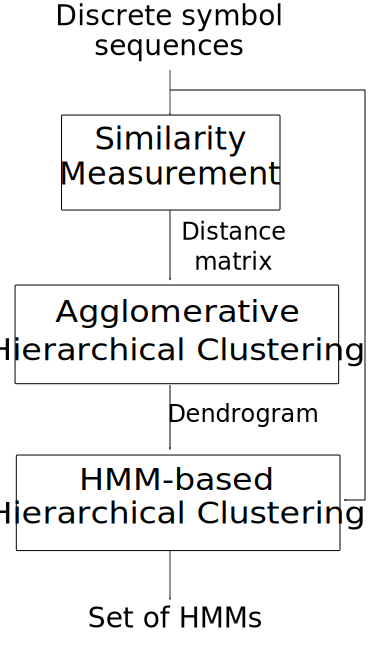
\includegraphics[height=2.5in]{figures/behavior-clustering-block-diagram}
            \caption{Block Diagram of Behavior Clustering}
            \label{fig:behavior-clustering-block-diagram}
        \end{center}
    \end{figure}
    
\end{frame}

%--------------------------------------------------------------------

\begin{frame}
    \frametitle{Clustering Human Behaviors}
    \framesubtitle{Processing Flow}
    
    \begin{figure}
        \begin{center}
            \includegraphics[height=2.8in]{figures/flow-diagram}
            \vspace{-0.2in}
            \caption{Processing flow of the use of HMM clustering method}
            \label{fig:processing-flow}
        \end{center}
    \end{figure}
    
\end{frame}

%--------------------------------------------------------------------

\begin{frame}
    \frametitle{Clustering Human Behaviors}
    \framesubtitle{Experimental Results}

    \begin{itemize}
        \item Recorded videos at a resolution of $320 \times 240$ 
            and 25 fps over 1 week.
        \item Used a motion detection to save disk space.
        \item Obtained videos corresponding to over 500 motion 
            events, but selected the 298 videos containing only 
            a single motion.
    \end{itemize}

\end{frame}

%--------------------------------------------------------------------

\begin{frame}
    \frametitle{Clustering Human Behaviors}
    \framesubtitle{Exerimental Results (cont.)}
    
    \begin{itemize}
        \item Found that at least 4 common behaviors:
            \begin{itemize}
                \item Walking into the building (Walk-in)
                \item Walking out of the building (Walk-out)
                \item Parking a bicycle (Cycle-in)
                \item Riding a bicycle out (Cycle-out)
            \end{itemize}
        \item Other less common activities:
            \begin{itemize}
                \item Walking while telephoning, etc. (Other)
            \end{itemize}
    \end{itemize}

\end{frame}

%--------------------------------------------------------------------

\begin{frame}
    \frametitle{Clustering Human Behaviors}
    \framesubtitle{Experimental Results (cont.)}
    
    \begin{figure}
        \centering
        \subfloat[]{\includegraphics[width=0.2\linewidth]{figures/example-behavior01}}
        \hspace{0.05in}
        \subfloat[]{\includegraphics[width=0.2\linewidth]{figures/example-behavior02}}
        \hspace{0.05in}
        \subfloat[]{\includegraphics[width=0.2\linewidth]{figures/example-behavior03}}
        \hspace{0.05in}
        \subfloat[]{\includegraphics[width=0.2\linewidth]{figures/example-behavior04}}
        \caption{Examples of common human activities in our 
            testbed scene. (a) Walking in. (b) Walking out. 
            (c) Cycling in. (d) Cycling out.}
        \label{fig:example-behavior}
    \end{figure}

\end{frame}

%--------------------------------------------------------------------

\begin{frame}
    \frametitle{Clustering Human Behaviors}
    \framesubtitle{Experimental Results (cont.)}
    
    \begin{block}{Our Main Hypothesis}
        \begin{itemize}
            \item Using DTW as a pre-process prior to HMM-based 
                clustering should improve the quality of the clusters 
                in term of separating anomalous from typical behaviors.
            \item Compared to
                \begin{itemize}
                    \item Using only HMMs
                    \item Supervised classification with HMMs
                \end{itemize}
        \end{itemize}
    \end{block}

\end{frame}

%--------------------------------------------------------------------

\begin{frame}
    \frametitle{Clustering Human Behaviors}
    \framesubtitle{Experimental Results (cont.)}

    \begin{itemize}
        \item Performed 3 experiments.
        \item Evaluated the results according to how well 
            the induced categories separate the anomalous 
            sequences (hand-labeled with the category ``Other'') 
            from typical sequences (Walk-in, Walk-out, Cycle-in, 
            Cycle-out).
            \begin{enumerate}
                \item Using our proposed method
                \item Using only HMMs 
                \item Using HMMs with supervised learning
            \end{enumerate}
        \item In all 3 experiments, we chose linear HMMs with 4 
            states based on our previous empirical experience.
    \end{itemize}

\end{frame}

%--------------------------------------------------------------------

\begin{frame}
    \frametitle{Clustering Human Behaviors}
    \framesubtitle{Experimental Results (cont.)}
    
    Our configuration
    
    \begin{itemize}
        \item the number of deviant patterns allowed in a cluster $N = 10$
        \item $z = 2.0$ for a threshold $p_c = \mu_c - z\sigma_c$
    \end{itemize}

\end{frame}

%--------------------------------------------------------------------

\begin{frame}
    \frametitle{Clustering Human Behaviors}
    \framesubtitle{Results for Experiment I (DTW+HMMs)}
    
    \centering Clustering results for Experiment I (DTW+HMMs).
    
    \begin{table}
        \vspace{-0.1in}
        \centering
        \begin{tabular}{ | c | c | c | c | c | c | }
            \hline
            Cluster \# & Walk-in & Walk-out & Cycle-in & Cycle-out & Other \\ \hline
            1 & 96 & 0 & 18 & 0 & 0 \\ \hline
            2 & 0 & 54 & 0 & 5 & 0 \\ \hline
            3 & 0 & 3 & 0 & 8 & 0 \\ \hline
            4 & 0 & 2 & 0 & 0 & 0 \\ \hline
            5 & 0 & 1 & 0 & 2 & 0 \\ \hline
            \multicolumn{6}{c}{...} \\ \hline
            14 & 0 & 0 & 0 & 0 & 4 \\ \hline
            15 & 0 & 0 & 0 & 0 & 4 \\ \hline
            16 & 0 & 0 & 0 & 0 & 2 \\ \hline
            17 & 0 & 0 & 0 & 0 & 2 \\ \hline
            One-seq & & & & & \\
            clusters & 4 & 17 & 34 & 21 & 4 \\ \hline
        \end{tabular}
    \end{table}
    
\end{frame}

%--------------------------------------------------------------------

\begin{frame}
    \frametitle{Clustering Human Behaviors}
    \framesubtitle{Results for Experiment II (HMMs only)}

    \begin{itemize}
        \item Begin by training a single HMM on all sequences.
        \item Assign every sequence with a per-observation log-likelihood 
            above a threshold $p_c$ to a cluster.
        \item Repeat the process by training a new HMM on the 
            remaining sequences.
    \end{itemize}

    \medskip

    \centering Clustering results for Experiment II (HMMs only).

    \begin{table}
        \label{tab:hmm-assoc-matrix}
        \vspace{-0.1in}
        \centering
        \begin{tabular}{ | c | c | c | c | c | c | }
            \hline
            Cluster \# & Walk-in & Walk-out & Cycle-in & Cycle-out & Other \\ 
            \hline 
            1 & 15 & 77 & 49 & 43 & 16 \\ \hline
            2 & 80 & 0 & 11 & 2 & 0 \\ \hline   
            3 & 5 & 0 & 0 & 0 & 0 \\ \hline 
        \end{tabular}
    \end{table}

\end{frame}

%--------------------------------------------------------------------

\begin{frame}
    \frametitle{Clustering Human Behaviors}
    \framesubtitle{Results for Experiment III (Supervised 
        Classification with HMMs)}

    \begin{itemize}
        \item Trained 4 HMMs on each of the four typical beahviors.
        \item Maximize the F1 value to determine the best per-observation 
            log-likelihood threshold for each HMM.
            \begin{itemize}
                \item For the best separation between the positive and 
                    negative test patterns
            \end{itemize}
    \end{itemize}

    \medskip
    
    \centering Results for Experiment III (Supervised classification with HMMs).
    
    \begin{table}
        \label{tab:hmm-supervised-classification}
        \vspace{-0.1in}
        \centering
        \begin{tabular}{ | c | c | }
            \hline
            Anomaly detection rate (\%) & False alarm rate (\%) \\ \hline
            50 & 24.6 \\ \hline
        \end{tabular}
    \end{table}

\end{frame}

%--------------------------------------------------------------------

\begin{frame}
    \frametitle{Clustering Human Behaviors}
    \framesubtitle{Conclusion}
    
    We have proposed and evaluated a new method for 
    clustering human behaviors.

    \medskip

    Our method
    \begin{itemize}
        \item provides an initial partitioning of a set 
            of behavior sequences, then automatically 
            identifies where to cut off the hierarchical 
            clustering dendrogram.
        \item could be used to bootstrap an anomaly 
            detection module for intelligent video surveillance 
            applications.
        \item shows a desirable separation between typical and 
            anomalous behaviors on real-world surveillance data 
            \alert{without} any information about the labels.
    \end{itemize}

\end{frame}

%--------------------------------------------------------------------

\begin{frame}
    \frametitle{Clustering Human Behaviors}
    \framesubtitle{Discussion}

    The combination of DTW with the type of linear HMMs we 
    use is very effective. 
    
    \bigskip
    
    It is likely that the patterns DTW groups together are 
    perfectly suited for modeling by this type of HMM. We 
    plan to further explore this idea in the future work.

    \bigskip 

    One limitation is that although the method achieves 100\% accuracy 
    in separating typical from anomalous events, it does so at the cost 
    of creating a fairly large number of single-sequence clusters that 
    would have to be manually identified as typical or anomalous by a 
    human operator in a real surveillance setting.

\end{frame}

%--------------------------------------------------------------------

\else

\begin{frame}
    \frametitle{Clustering Human Behaviors}
    \framesubtitle{Conclusion}
    
    We have proposed and evaluated a new method for 
    clustering human behaviors.

    \medskip

    Our method
    \begin{itemize}
        \item provides an initial partitioning of a set 
            of behavior sequences, then automatically 
            identifies where to cut off the hierarchical 
            clustering dendrogram.
        \item could be used to bootstrap an anomaly 
            detection module for intelligent video surveillance 
            applications.
        \item shows a desirable separation between typical and 
            anomalous behaviors on real-world surveillance data 
            \alert{without} any information about the labels.
    \end{itemize}

\end{frame}

%--------------------------------------------------------------------

\begin{frame}
    \frametitle{Clustering Human Behaviors}
    \framesubtitle{Discussion}

    The combination of DTW with the type of linear HMMs we 
    use is very effective. 
    
    \bigskip
    
    It is likely that the patterns DTW groups together are 
    perfectly suited for modeling by this type of HMM. We 
    plan to further explore this idea in the future work.

    \bigskip 

    One limitation is that although the method achieves 100\% accuracy 
    in separating typical from anomalous events, it does so at the cost 
    of creating a fairly large number of single-sequence clusters that 
    would have to be manually identified as typical or anomalous by a 
    human operator in a real surveillance setting.

\end{frame}

\fi

